\chapter{Church-Turing Tese}

De maskiner vi har kigget på indtil videre har enten været med endelig hukommelse (Endelige Automater) eller med en uendelig hukommelse der kun fungerer i en LIFO stak-hukommelse (PDA). Dermed er de for begrænset til at kunne agere som modeller af almene computere, da disse har ubegrænset, uendelig hukommelse.

\section{Turingmaskiner}%
\label{sec:turingmachines}

I 1936 introducerede Alan Turing \textit{turingmaskinen}, en deterministisk model som minder om en endelig automat, men med uendeligt og ubegrænset hukommelse. Denne model af en maskine kan alt det som en almen computer\footnote{Her bruges ``almen computer'' som en oversættelse fra det engelske ``General Purpose Computer''} kan gøre. Dermed kan vi bruge denne model til at finde ud af begrænsninger m.m. om de computere vi bruger i dagligdagen.

En turingmaskine bruger et uendeligt bånd som dets hukommelse. Den har en \textit{båndhoved} som kan læse \textit{og skrive} symboler og flytte sig selv rundt på båndet. Til at starte med indeholder båndet kan input strengen, dog kan den skrive på dette bånd. Til at læse informationen går båndhovedet over de symboler der skal læses. Maskinen bliver ved med at komputere indtil den vælger at producere et output, enten \textit{accept} eller \textit{afvis}. Hvis den ikke kommer til et accept eller afvis state, så kører den for evigt, uden nogensinde at stoppe. Når komputeringen rammer en af disse states, stopper komputeringen.

\begin{figure}[ht]
	\centering
	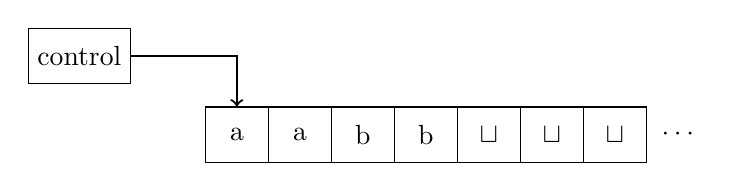
\begin{tikzpicture}
		\tikzset{block/.style={rectangle, draw, minimum height=2em, minimum width=3em}}
		\tikzset{line/.style={draw, -latex'}}
		\node[block] (control) {control};

		\node[block, minimum width=0.8cm] (a1) at (2,-1.0) {a};
		\node[block, minimum width=0.8cm] (a2) at (2.8,-1.0) {a};
		\node[block, minimum width=0.8cm] (b1) at (3.6,-1.0) {b};
		\node[block, minimum width=0.8cm] (b2) at (4.4,-1.0) {b};
		\node[block, minimum width=0.8cm] (b2) at (5.2,-1.0) {$\sqcup$};
		\node[block, minimum width=0.8cm] (b2) at (6.0,-1.0) {$\sqcup$};
		\node[block, minimum width=0.8cm] (b2) at (6.8,-1.0) {$\sqcup$};
		\node[label, minimum width=0.8cm] (b2) at (7.6,-1.0) {$\cdots$};

		\draw[->, thick] (control) -| (a1);
	\end{tikzpicture}
	\caption{\label{fig:turingschematic} Skematik af en turingmaskine.}
\end{figure}
I Figur~\ref{fig:turingschematic} kan der ses en skematik på en turingmaskine. Læg her mærke til at båndet er uendeligt langt, og efter input strengen er der bare blanke symboler, her betegnet som $\sqcup$.

Følgende punkter opsummerer forskellen mellem en endelig automat og en turingmaskine:

\begin{enumerate}
	\item En Turingmaskine kan både læse og skrive fra båndet.
	\item Læs-skriv (read-write) hovedet kan bevæge sig både til athøjre og til venstre.
	\item Båndet er uendeligt.
	\item De speceielle states til at acceptere og afvise et input træder i kraft med det samme.
\end{enumerate}



\subsection{Formel Definition af en Turingmaskine}%
\label{subsec:formaldefturingmachine}



Trods vi næsten aldrig bruger den formelle beskrivelse af en turingmaskine, da de oftest ender med at blive alt for store, giver vi den generelle formelle beskrivelse af en turingmaskine her.

Transitionsfunktionen i en turing maskine har formen $Q \times \Gamma \longrightarrow Q \times \Gamma \times \{L, R\}$. For eksempel betyder $\delta (q,a) = (r,b,L)$ at når båndet er over symbol $a$ og maskinen er i state $q$, så skal den skrive $b$ til symbolet hvor $a$ tidligere stod, og gå til state $r$. $L$ betyder her at den skal bevæge sig til venstre.

\begin{definition}[Formel Definition af en Turingmaskine]
	\label{def:formalturing}
	En \textbf{Turingmaskine} er en 7-tuple $(Q, \Sigma, \Gamma, \delta, q_{0}, q_{\text{accept}}, q_{\text{reject}})$, hvor $Q, \Sigma, \Gamma$ alle er endelige sæt, og
	\begin{enumerate}
		\item $Q$ er sættet af states.
		\item $\Sigma$ er inputalfabetet ikke indeholdende det blanke symbol, $\sqcup$.
		\item $\Gamma$ er båndalfabetet, hvor $\sqcup \in \Gamma$ og $\Sigma \subseteq \Gamma$.
		\item $\delta, Q \times \Gamma \longrightarrow Q \times \Gamma \times \{L, R\}$ er transitionsfunktionen.
		\item $q_{0} \in Q$ er startstaten.
		\item $q_{\text{accept}} \in Q$ er accept staten.
		\item $q_{\text{reject}} \in Q$ er afvis staten, hvor $q_{\text{accept}} \neq q_{\text{reject}}$.
	\end{enumerate}
\end{definition}

Bemærk at, på trods af at Sipser ikke skriver det som en mulighed, kan man nemt implementere ``stay'' (her skrevet S) som en mulighed, fromfor kun at vælge left eller right. Du kan gøre dette ved at først skrive, så gå til højre, så gå til venstre uden at gøre noget med symbolet.


\subsection{Turingmaskine Komputering}%
\label{subsec:turingmaskinekomputering}

En turingmaskine komputere ved at starte sit båndhoved på den venstremest symbol på båndet. Inputtet $w = w_{1}w_{2} \ldots w_{n} \in \Sigma^{*}$ er på de første (venstremest) $n$ pladser på båndet, og det resterende er blankt. Siden $\Sigma$ ikke indeholder de blanke symbol, kan man være sikker på at så snart det blanke symbol kommer på båndet, har man læst inputtet færdigt. Hvis hovedet nogensinde forsøger at bevæge sig mere til venstre end muligt, så forbliver hovedet på den venstremest symbolplacering, trods den ``skal'' gå til venstre. Når $M$ er begyndt bevæger den sig efter reglerne beskrevet i transitionsfunktionen, indtil den enten accepterer eller afviser inputtet og dermed stopper. Hvis den hverken accepterer eller afviser inputtet kører den forevigt.


I Figur~\ref{fig:turingcomputation} ses hvordan båndindholdet, hovedet, og staten ændrer sig fra en state til en anden, givet reglen $\delta(q_{i}, c) = (q_{j}, x, L)$.

\begin{figure}[ht]
	\centering
	\begin{tikzpicture}
		\tikzset{block/.style={rectangle, draw}}
		\tikzset{line/.style={draw, -latex'}}

		% Define starting position
		\def\startx{0}
		\def\gap{0.8} % Gap between each block


		\node[draw=none, fill=none] at (-1.4, -0.2) { \begin{tabular}{c}Venstre $\rightarrow$\\Ende\end{tabular} };
		% Labels for each block, can add/remove as needed
		\def\labels{a, a, a, b, b, b, c, $\sqcup$, $\ldots$, $\sqcup$}

		% Foreach loop to create nodes automatically
		\foreach \label [count=\i] in \labels {
			\node[block, minimum width=0.8cm, minimum height=0.8cm] (block\i) at (\startx + \gap*\i - \gap,0.0) {\label};
		}

		\node[block, minimum width=1.0cm, minimum height=1.0cm, draw=SchemeRed, line width=0.40mm] (reading) at (2.4, 0.0) {};
		\node[draw=none, fill=none, text=SchemeRed] at (2.4, -0.7) { Hovedet };
		\node[draw=none, fill=none] at (8.0, 0.0) {$\rightarrow \infty$};
		\node[draw=none, fill=none, text=SchemeBlue] at (5.4, -0.7) { State $q_{i}$ };
		\node[draw=none, fill=none] at (5.4, -1.7) { $\Downarrow$ \hspace{1cm} $\delta(q_{i},c) = (q_{j}, x, L)$ };


		\def\labelstwo{a, a, a, x, b, b, c, $\sqcup$, $\ldots$, $\sqcup$}

		% Foreach loop to create nodes automatically
		\foreach \label [count=\y] in \labelstwo {
			\node[block, minimum width=0.8cm, minimum height=0.8cm] (block\y) at (\startx + \gap*\y - \gap,-3.0) {\label};
		}
		\node[block, minimum width=1.0cm, minimum height=1.0cm, draw=SchemeRed, line width=0.40mm] (reading) at (1.6, -3.0) {};
		\node[draw=none, fill=none, text=SchemeRed] at (1.6, -3.7) { Hovedet };
		\node[draw=none, fill=none] at (8.0, -3.0) {$\rightarrow \infty$};
		\node[draw=none, fill=none, text=SchemeBlue] at (5.4, -3.7) { State $q_{j}$ };
	\end{tikzpicture}
	\caption{\label{fig:turingcomputation} Komputering i en Turingmaskine.}
\end{figure}

En \textit{konfiguration} er en kombination af de følgende tre ting:
\begin{itemize}
	\item Den nuværende state.
	\item Det nuværende indhold af båndet.
	\item Hovedet nuværende lokation.
\end{itemize}

De her konfigurationer bliver oftest repræsenteret på følgende måde: Givet en state $q$ og to strenge $u$ og $v$ over båndalfabetet $\Gamma$, skriver vi $uqv$ for konfigurationen hvor den nuværende state er $q$, båndindholdet er $uv$ og hovedets lokation er ved det andet symbol, altså $v$.

Vi siger at en konfiguration $C_{1}$ \textit{giver} konfigurationen $C_{2}$ hvis turingmaskinen lovligt kan gå fra $C_{1}$ til $C_{2}$ på et enkelt skridt.

\textit{Startkonfigurationen} af $M$ på input $w$ er konfigurationen $q_{0}w$. Altså hvor staten er helt i start, og resterende af strengen, $w$ efterfølger. I en \textit{accepterende konfiguration} er staten i en konfiguration $q_{\text{accept}}$. I en \textit{afvisende konfiguration} er staten $q_{\text{reject}}$. Accept og afvisekonfigurationer er \textit{standsende konfigurationer}, altså konfigurationer som ikke giver flere konfigurationer.

Vi kalder samlingen af strenge som $M$ accepterer \textit{sproget af $M$} eller \textit{sproget genkendt af $M$}, betegnet $L(M)$.

\begin{definition}
	Kald et sprog \textit{Turing-genkendeligt} hvis en Turingmaskine genkender det.
\end{definition}

Dette kan også beskrives $L(m) = \{w \mid q_{0}w \stackrel{*}{\Rightarrow} uq_{\text{acc}}v \text{ for nogen }u,v \in \Gamma^{*}\}$

Når en turingmaskine startes er tre resultater mulige, enten vil maskinen \textit{acceptere}, \textit{afvise} eller \textit{løkke}\footnote{\textit{loop} på engelsk}, hvor \textit{løkke} betyder at maskinen vil køre forevigt.


Vi kalder maskiner der aldrig kommer i en løkke for beslutningstagere eller afgørerere\footnote{Måske? Deciders på engelsk.}, fordi de altid afgører hvorvidt en streng skal accepteres eller afvises. En afgører som genkender et sprog, siges også at \textit{afgøre} det sprog.

\begin{definition}
	Kald et sprog Turing-afgjort eller simpelt afgjort, hvis en turingmaskine afgører (beslutter) det.
\end{definition}

Dette kaldes også \textit{rekursivt enumerabelt\footnote{Engelsk: recursively enumerable}} i litteraturen.

\begin{figure}[ht]
	\centering
	\begin{tikzpicture}
		\draw[SchemeLight,fill=SchemeLight,dashed, thick, opacity=0.2] (0.5,0) ellipse (4cm and 2cm);
		\draw node at (1.7,1) {Genkendelige sprog};
		\draw[SchemeBlue,fill=SchemeBlue,dashed, thick, opacity=0.5] (-1.0,0) ellipse (2cm and 1.0cm);
		\draw node at (-1,0) {Afgørlige sprog};
	\end{tikzpicture}
	\caption{\label{fig:univers} Univers af sprog}
\end{figure}

I figur~\ref{fig:univers} ses der hvordan de afgørlige sprog kun er en delmængde af alle de genkendelige sprog. Under de afgørlige sprog ligger også kontekstfrie sprog og regulære sprog.

\section{Varianter af Turingmaskiner}%
\label{sec:turingvariants}

Vi kalder andre versioner af turingmaskinen, herunder maskiner med flere bånd eller nondeterministiske maskiner for \textit{varianter}. Den originale model og alle dens varianter har samme deskriptive kraft. Vi kalder dette \textit{robusthed}, altså, at maskinerne alle beskriver samme klasse af sprog.

\subsection{Multibånds Turingmaskiner}%
\label{subsec:multitape}

En \textbf{multibånds turingmaskine} er som en normal turingmaskine, men med mere end ét bånd (hvor antallet \textbf{ikke} må ændres under kørsel.) Transitionsfunktionen ændres så den kan køre på mere end ét bånd:
\[ \delta : Q \times \Gamma^{k} \longrightarrow Q \times \Gamma^{k} \times \{L,R,S\}^{k}\] hvor $k$ er antallet af states. Dermed fungerer transitionsfunktionen ved at tage den nuværende state i alle tapes og giver resultatet i alle states, eksempelvis: $\delta(q_{i}, a_{1}, \ldots, a_{k}) = (q_{j}, b_{1}, \ldots, b_{k}, L, R, \ldots, L)$, hvor $b_{i}$ erstatter $a_{i}$, når hovedet bevæges. Jørgens implementation af multibåndsmaskinen har også $\gamma_{j} \in \{L, R, S\}$, altså, hvor han tillader hovedet at stå stille.

En multibånds turingmaskine kan være meget brugbar, ved at gøre ting mere intuitivt nemme at forstå (på samme måde som en NFA.) Et godt eksempel på dette er kopiering af en streng. Følgende algoritme vil fungere til \textbf{alle} $k-$bånds turingmaskiner, hvor $k \ge 2$. Lad $m$ være maskinen, der kopierer sit input $w$.

Lad $m$ på input $w$:
\begin{enumerate}
	\item For hvert bogstav i bånd 1, kopiér dette ned til bånd 2.
	\item Flyt hovedet i bånd 1 til første tomme symbol, $\sqcup$.
	\item Kopiér fra bånd 2 symbol-pr-symbol til bånd 1, start ved hovedets lokation.
	\item Fjern indhold i bånd 1.
\end{enumerate}

Dette kan gøres i $O(|w|)$ skridt, imens den kan gøres i $O(|w|^{2})$ skridt i en 1-båndsmaskine. Altså er det en væsentlig hurtigere måde at gøre det på, men begge kører alligevel i polynomiel tid.


\begin{theorem}
	\label{teo:multitapeequiv}
	Hver multibånds turingmaskine har en ækvivalent enkeltbånds turingmaskine.
\end{theorem}

\begin{proof}
	For at bevise dette, skal vi vise at enhver multibånds Turingmaskine $M$ kan konverteres til en enkeltbånds Turingmaskine $S$. Vi siger at $M$ har $k$ bånd. Så bruger $S$ symbolet \# til at indikere at et nyt bånd starter. Derudover skal $S$ også holde styr på lokationen af hovederne fra diverse bånd. Den gør dette ved at skrive en bolle over symbolet: $\mathring{b}$.

	Så en maskine med tre bånd som f.eks.:\\
	\begin{center}
		\noindent
		\texttt{\textbf{a}aaaabababbb}\\
		\noindent
		\texttt{bbbbb\textbf{b}bbbbba}\\
		\noindent
		\texttt{a\textbf{b}aaababbaba}\\
	\end{center}
	Hvor \textbf{tyk skrift} indikerer hovedets placering, bliver lavet om til i $S$:
	\begin{center}
		\texttt{$\stackrel{\circ}{\text{\texttt{a}}}$aaaabababbb\#bbbbb$\stackrel{\circ}{\text{\texttt{b}}}$bbbbba\#a$\stackrel{\circ}{\text{\texttt{b}}}$aaababbaba\#}.
	  \end{center}

	Vi definerer nu $S$.

	$S = $ ``På input $w = w_{1} \cdots w_{n}$'':
	\begin{enumerate}
		\item Først konverterer $S$ til enkeltbånd.
		\item Til at simulere en enkelt bevægelse, scanner $S$ fra den første \# til $k+1$'e \#, som er slutningen i højresiden, så den kan finde ud af hvad symbolerne under de virtuelle hoveder er. Så laver $S$ en til passthrough til at opdatere ifølge reglerne. Hvis på noget tidpsunkt, $S$ vil flytte til højre til et $\#$ (altså, hvad der i det originale bånd er $\sqcup$), så rightshifter $S$ alt derfra, så vi får ekstra plads, til hvor der ville være et blankt symbol. På samme måde kan vi leftshifte, hvis det er en nødvendighed.
	\end{enumerate}

	Altså vil alle symboler med en bolle over agere som hovederne på et normalt bånd, hvor hovedet så simulerer hvad reglerne er for hver af båndene.
\end{proof}

Vi kan i beviset tydeligt se hvordan det kan gøres, men hvordan kan en simulerende Turingmaskine som $S$ huske at den har set de tidligere hoveder? Følgende er en beskrivelse af en algoritme der kan konvertere enhver $k-$bånds Turingmaskine til en $1-$bånds Turingmkasine.

\begin{enumerate}
  \item Antag at $M$ er en $k-$bånds Turingmaskine.
  \item For hver state $q_{i}$ i $M$ har vi:
		\begin{enumerate}
		  \item\label{enum:ktapealgo:qi} States $q^{i}_{(\alpha_{1}, \alpha_{2}, \ldots, \alpha_{k})}$ når $a_{i} \in \Gamma \cup \{-\}$, hvor $-$ betyder tomme eller endnu ikke kendt, altså, vi ved endnu ikke hvad der skal være der.
		  \item\label{enum:ktapealgo:pi} States $p^{i}_{(\delta_{1}, \delta_{2}, \ldots, \delta_{k}, b_{1}, b_{2}, \ldots, b_{k}, \gamma_{1}, \gamma_{2}, \ldots, \gamma_{k})}$ hvor $\delta_{i} \in \Gamma \cup \{-\}$, $b_{i} \in \Gamma$, $\gamma_{i} \in \{R, L, S\}$. Så altså, det første (\(\delta\)) er enten båndsymboler eller ukendt, $b$  er båndsymboler,  og $\gamma$ er hovedbevægelser.
		\end{enumerate}
\end{enumerate}

For at forklare dybere: \ref{enum:ktapealgo:qi}: Når vi er i $q^{i}_{(\beta_{1}, \beta_{2}, \ldots, \beta_{r},-,-,\ldots,-)}$ har vi indsamlet alle symbolerne under hovederne på de første $r$ bånd. Her betyder symbolerne $-$ igen at det er symboler som vi ikke kender endnu. Altså betyder det at \(\beta_{k}\) har hvad det simulerer bånd nummer $k$'s symbol under hovedet.
\ref{enum:ktapealgo:pi}: Når vi er i $p^{i}_{(b_{1}, \ldots, b_{q}, -, \ldots, -, b_{1}, b_{2}, \ldots, b_k, \gamma_{1}, \gamma_{2}, \ldots, \gamma_{k})}$ har vi ændret båndcellerne under de første $q$ hoevbder og flyttet den $i'$e hoved $i \le q$ ifølge $\gamma_{i}$ og muligvis rightshifted. Altså, når vi er i den state, har vi allerede erstattet $a_{1}, \ldots, a_{q}$ med $b_{1}, \ldots, b_{q}$ og vi har flyttet hovederne ifølge reglerne $\delta_{1}, \ldots \delta_{k}$.

Vi kan her se at der  er mange af de mulige states beskrevet i \ref{enum:ktapealgo:pi} og \ref{enum:ktapealgo:qi}. Til $q^{i}$ er der $(\Gamma+1)^{k}$ (fordi der er $k$ states, og $\Gamma$ symboler eksklusiv $-$). Til $p^{i}$ er det $(\Gamma+1)^{k} + \Gamma^{k} + 3^{k}$. Altså er der utroligt mange mulige states.

Altså kan man se det totale antal af states som en \textbf{endelig} funktion $f(k, \Gamma, Q)$. Altså er antallet af states polynomielt, og \textbf{ikke} eksponentielt, da $k$ er en konstant.

Lad os nu implementere ét skridt $\delta(q_{i}, a_{1}, a_{2}, \ldots, a_{n}) = (q_{j}, b_{1}, b_{2}, \ldots, b_{k}, \gamma_{1}, \gamma_{2}, \ldots, \gamma_{k})$.
\begin{enumerate}
  \item $M'$ starter i state $q^{i}_{(-,-, \ldots, -)}$ på den venstremest position altså uden kendskab til nogen symboler.
  \item I state $q^{i}(a_{1}, \ldots, a_{r}, -, \ldots, -)$ $r < k$, flytter $m'$ dets hoved fremad til at kopiere indholdet under $m'$s $(r+1)$'e hoved. Vi husker så via. staten, altså, når vi har set symbol $a$ under det $i$'e hoved, så går vi til den state der har symbol $a$ under det $i$'e hoved. Det er måden vores hukommelse fungerer på.
  \item Når vi når til state $q^{i}_{(a_{1}, a_{2}, \ldots, a_{k})}$ $\beta_{i} \in \Gamma$ har vi samlet alle karakterer under $m'$s hoveder. Så er det tid til at ændre på disse symboler. Jævnfør algoritmen vi har set tidligere gør vi dette ved hjælp af en ``mellem-state'', $p^{j}$ (hvor vi egentlig gerne vil hen til $q_{j}$.) Vi går til state $p^{j}_{(-, \ldots, -, b_{1}, b_{2}, \ldots, b_{k}, \gamma_{1}, \gamma_{2}, \ldots, \gamma_{k})}$ hvor vi endnu ikke ved hvad de første symboler der skal ændres er, men vi ved hvad de skal ændres \textit{til} (fra transitionsfunktionens definition skrevet lige før starten på denne implementation.)
  \item I state $p^{j}_{(b_{1}, \ldots, b_{s}, -, \ldots, -, b_{1}, b_{2}, \ldots, b_{k}, \gamma_{1}, \gamma_{2}, \ldots, \gamma_{k})}$ hvor $s < k$ gør vi følgende:
		\begin{enumerate}
		  \item Flytter til positionen af det $(s+1)$'e hoved.
		  \item Erstatter $a_{s+1}$ med $b_{s+1}$ og flytter ``hovedet'' $s+1$ ifølge $\gamma_{s+1}$
		  \item Hvis $s+1<k$ går vi til state $p^{j}_{(b_{1}, \ldots, b_{s+1}, \cdots, b_{1}, b_{2}, \ldots, b_{k}, \gamma_{1}, \ldots, \gamma_{k})}$, og tager skridt 4 om igen. \textbf{Ellers} flytter vi hovedet til den venstremest position og går til state $q^{j}_{(-, \ldots, -)}$
		\end{enumerate}
\end{enumerate}

Hvad er \textbf{køretiden} så for denne simulation? Givet en afgørlig Turingmaskine (altså, der stopper), som tager $t$ skridt på input $w, |w| = n$. Båndet i denne Turingmaskine kan have højest længde $n + t$, da den starter med input $n$, og højest kan lave $t$ ændringer til båndet der gør den længere. Lad os forsøge at ræssonere os frem til køretiden. Vi kører frem og tilbage i båndet flere gange, for hvert skridt kører vi frem én gang, så kører vi tilbage, og så kører vi frem (hvor vi udfører transitionsfunktionen); og så tilbage. Altså gør vi det fire gange. Dermed har ét skridt køretid $O(\Sigma \text{ længden af båndet}) = O(n+kt)$, hvor $k$ er antal bånd. Derudover er det muligt, at vi skal lave flere \textit{rightshifts}. I worst case scenariet shifter vi hver gang, hvilket giver os $(k-1)t + (k-2)t + \cdots + t = O(k^{2}t)$. Dermed er det samlede arbejde gjort på ét skidt $O(n+kt)+O(k^{2}t) = O(n+k^{2}t)$. Da vi har $t$ skridt, vil det samlede arbejde for at simulere disse skridt være $O(n \cdot t + k^{2}t^{2})$, hvilket er polynomielt i $n$ og $t$.




\begin{corollary}
	Et sprog er Turing-genkendeligt hvis og kun hvis en multibånds Turingmaskine genkender det.
\end{corollary}

\begin{proof}
	En Turingmaskine er genkendt af en multibåndsmaskine med ét bånd. Den anden vej bevises i Teorem~\ref{teo:multitapeequiv}.
\end{proof}


\subsection{2-vejs bånd}
\label{subsec:2vejsbånd}

Denne variant minder om en normal, deterministisk turingmaskine. Dog har den en ekstra egenskab: nemlig at den også er uendelig på venstresiden. I Figur~\ref{fig:2vejsbånd} ses en skitse af hvordan en 2-vejs bånds Turingmaskine ser ud.

\begin{figure}[ht]
	\centering
	\begin{tikzpicture}
		\tikzset{block/.style={rectangle, draw}}
		\tikzset{line/.style={draw, -latex'}}

		% Define starting position
		\def\startx{0}
		\def\gap{0.8} % Gap between each block


		% Labels for each block, can add/remove as needed
		\def\labels{ ,  ,  ,  ,  ,  ,  , , }
		\def\indices{-4,-3,-2,-1,0,1,2,3,4}

		% Foreach loop to create nodes automatically
		\foreach \label [count=\i] in \labels {
			\node[block, minimum width=0.8cm, minimum height=0.8cm] (block\i) at (\startx + \gap*\i - \gap,0.0) {\label};
		}
		\foreach \label [count=\y] in \indices {
			\node[draw=none, fill=none, minimum width=0.8cm, minimum height=0.8cm,color=SchemeRed] (block\y) at (\startx + \gap*\y - \gap,0.7) {\label};
		}

		\node[draw=none, fill=none] at (7.2, 0.0) {$\rightarrow \infty$};
		\node[draw=none, fill=none] at (-0.8, 0.0) {$\infty \leftarrow$};

	\end{tikzpicture}
	\caption{\label{fig:2vejsbånd} 2-vejs bånd variant.}
\end{figure}


\subsection{Nondeterministisk Turingmaskine}%
\label{subsec:nondeterministicturingmachine}

En nondeterministisk turingmaskine fungerer nondeterministisk ligesom PDA og NFA. Altså kan den gætte fra et state $q$, hvad den skal gøre som det næste. Dette betyder også at der er $B = |Q| \cdot |\Gamma| \cdot 3$ mulige transitioner.
Den brancher ud for hver mulighed. Transitionsfunktionen beskrives således:
\[ \delta : Q \times \Gamma \longrightarrow P(Q \times \Gamma \times \{L, R, S\})\]\footnote{Sipser bruger ikke $S$ som mulighed for at bevæge sig.}
Man kan se komputeringen som en træ-struktur, hvor hver gang den gætter, kommer der en ny gren på. Hvis en af de her grene ender i en accept state, så accepteres inputtet. Det er vigtigt at bemærke at hver transition, $\delta(q,a)$ har et endeligt antal, $B$, af mulige transitions, da $B \le |Q| \cdot |\Gamma| \cdot 3$.

Vi kalder en nondeterministisk turingmaskine en \textbf{afgører} hvis den stopper på alle grene.

Hvordan kan dette så være brugbart? For eksempel kan en nondeterministisk turingmaskine nemt finde ud af om $n$ er et sammensat tal (altså, ikke et primtal.) Den gør dette ved at have et heltal $n > 1$, og så gætter på alle tal om $m = n_{1} \cdot n_{2}$, ved at udregne deres værdi, og sætte lighed mellem denne og $n$.


\begin{definition}
  \label{def:ndtmrecog}
En nondeterministisk Turingmaskine (NDTM) $m$ \textbf{genkender} $L$ hvis $L = \{w \mid \exists \text{ en komputering for }M \text{ på } w \text{ der leder til } M \text{'s accept state} \}$
\end{definition}

\begin{definition}
  \label{def:ndtmdecide}
  En nondeterministik Turingmaskine $m$ \textbf{afgører} $L$ hvis $\forall w \in \Sigma^{*}$:
  \begin{enumerate}
	\item $\exists k = k(m,w)$ således at $m$ aldrig tagere mere end $k$ skridt på $w$, altså alle længder i træet har længde $\leq k$.
	\item $w \in L \iff m$  har mindst én accepterende beregning på $w$. Altså betyder det ikke at $w$ skal accepteres, men at hvis den accepteres, er den i sproget, og omvendt.
  \end{enumerate}
\end{definition}

Forskellen på Definitionerne \ref{def:ndtmrecog} og \ref{def:ndtmdecide} er at en Turingmaskine der genkender \textbf{tillader} uendelige veje, så længe der er en accept state, hvor en afgørende Turingmaskine \textbf{ikke} tillader uendelige veje.

\begin{theorem}
	\label{teo:nondeterminismturingequiv}
	Hver nondeterministisk turingmaskine har en ækvivalent deterministisk Turingmaskine.
\end{theorem}

Givet en deterministisk Turingmaskine $D$ der er ækvivalent til den nondeterministiske Turingmaskine $N$ gælder det at $L(D) = L(M)$ og $D$ afgører $L \iff N$ afgører $L$.

Vi vil gerne bevise ved at have en deterministisk turingmaskine $D$ til at simulere alle grene der er mulige v.h.a. nondeterminisme. Vi designer $D$ til at bruge breadth-first-search til at kigge alle grene igennem.

Vi vil gerne bruge \textit{breadth-first search} til at simulere $N$ på $w$. Vi ved at dette er muligt, fordi der ved hver state er \textbf{højest} $B$ transitions. Til gengæld vil vi ikke kunne gøre det med depth-first, da uendelige veje er mulige i træet.

Vi antager her at hver transition, $\delta(q,a)$ har \textbf{præcis} $B$ transitioner, eller ingen. Vi kan klare dette ved at kopiere den sidste state det antal gange der skal til, for at antallet af transitions bliver til $B$; e.g, hvis $B = 4$, og $\delta(q,a) = \{(q, b, R)\}$ så ændrer vi den til at være $\delta(q,a) = \{(q,b,R),(q,b,R),(q,b,R),(q,b,R)\}$

For en given streng $g_{1}g_{2}\cdots g_{k}$ hvor $g_{i} \in \{1, 2, \ldots, B\}$ kan vi simulere den korresponderende komputering af $N$  ved at tage det $g_{i}$'e valg på skridt $i$. Altså er en mulig streng 274, hvilket betyder at vi i første skridt tager valg nummer 2, i det andet valg nummer 7, og i det tredje valg nummer 4 (her er $B \ge 7$, da 7 er det største tal i strengen.) Hvis vi kan implementere simulationen beskrevet her ved en deterministisk Turingmaskine $D$, så opfylder $D$ Teorem~\ref{teo:nondeterminismturingequiv}.

Måden vi kigger komputeringerne igennem på er ved at gå lexicografisk igennem dem. Altså starter vi med alle strenge af længde én, og derefter længde to etc. Vi kører igennem de ``første'' tal først, så altså først 123, så 124, så 149 etc. Vi bliver ved med at gøre det på denne måde indtil vi finder en accepterende konfiguration.

Vi kan holde styr på tallene ved at bruge båndet i turingmaskinen. For eksempel kan strengen 223 blive repræsenteret således:
\begin{center}
\texttt{\#00\#00\#000\#}
\end{center}
Hvor den første del har to 0'er, den anden del har også to 0'er, og den tredje har tre 0'er.

Lad os nu kigge på hvordan vi faktisk laver den deterministiske Turingmaskine $D$ som simulerer $N$.
$D$ vil have 3 bånd:
\begin{enumerate}
  \item Input.
  \item $N$'s udregninger på $w$.
  \item Tal base $B+1$.
\end{enumerate}

For eksempel:
\begin{enumerate}
  \item $w_{1}w_{2} \cdots w_{n}$
  \item Simulering i 3 skridt i henhold til skridt 3.
  \item 235
\end{enumerate}

Hvis vi når til en komputering der ikke eksisterer (da vi går dem alle igennem), så stopper vi udregningen og går videre til næste mulighed.
Bemærk her at hvis $N$ er i en accepting state, så vil $D$ også acceptere input. På samme måde, hvis $N$ er en afgører, og $D$ har været \textbf{alle} states igennem, og endnu ikke fundet et accepting state, så bliver input afvist.

Lad os formalisere, og dermed færdiggøre beviset til Teorem~\ref{teo:nondeterminismturingequiv}:

\begin{proof}
\begin{enumerate}
  \item \begin{enumerate}
		  \item $w_{1}w_{2}\cdots w_{n}$
		  \item $\sqcup$
		  \item $\#0\#$
		\end{enumerate}
  \item Kopiér bånd 1 til bånd 2
  \item Simulér $N$ på bånd 2 ved brug af tallene på bånd 3 til at vælge den næste transition indtil følgende sker:
		\begin{itemize}
		  \item Dead end
		  \item $M$ accepteres, så vil $D$ også acceptere og stoppe udregning
		  \item $M$ afviser
		  \item Der ikke er flere tal på bånd 3
		\end{itemize}
  \item Erstat $d_{1},d_{2},\ldots, d_{r}$ på bånd 3 med det næste i leksikografisk orden
  \item Gå til skridt 2.
\end{enumerate}
\end{proof}


\begin{corollary}
	Et sprog er turing-genkendeligt hvis og kun hvis en nondeterministisk Turingmaskine genkender det.
\end{corollary}

\begin{proof}
	Enhver deterministisk Turingmaskine er automatisk også en nondeterministisk turingmaskine. Den anden retning følger fra~\ref{teo:nondeterminismturingequiv}.
\end{proof}

Hvor lang tid tager denne simulation af $N$ for $D$? Hvis vi antager at $N$ kører i $r$ skridt (altså, $r$ beregninger), så vil $D$ højest simulere
\begin{equation}
B+B^{2}+\cdots +B^{r} \leq B^{r+1}
\end{equation}
Altså vil den køre i \textbf{eksponentiel tid}. Dette kommer fra at der kan være $B$ udregninger i strengen af længde 1, $B^{2}$ af strengen af længde 2, etc\footnote{``Strengen'' her betyder den udregning vi er nået til, som brugt i bevisidéen til Teorem~\ref{teo:nondeterminismturingequiv}}.

\textbf{Hvis vi kunne lave en algoritme} der konverterer en nondeterministisk Turingmaskine til en deterministisk Turingmaskine som kører i polynomiel tid, ville vi bevise $P = NP$\footnote{Vi kommer ind på dette senere i kurset.}.

\subsection{Et bånd med flere hoveder}%
\label{subsec:etbåndflerehoveder}

\begin{figure}[ht]
	\centering
	\begin{tikzpicture}
		\tikzset{block/.style={rectangle, draw}}
		\tikzset{line/.style={draw, -latex'}}

		% Define starting position
		\def\startx{0}
		\def\gap{0.8} % Gap between each block


		% Labels for each block, can add/remove as needed
		\def\labels{ ,  ,  ,  ,  ,  ,  , , }

		% Foreach loop to create nodes automatically
		\foreach \label [count=\i] in \labels {
			\node[block, minimum width=0.8cm, minimum height=0.8cm] (block\i) at (\startx + \gap*\i - \gap,0.0) {\label};
		}

		\node[draw=none, fill=none] at (7.2, 0.0) {$\rightarrow \infty$};

		\node[block, minimum width=1.0cm, minimum height=1.2cm, draw=SchemeRed, line width=0.4mm] (h1) at (1.6, 0.0) {};
		\node[draw=none, fill=none, text=SchemeRed] (h1t) at (1.6, -1.0) {$h_{1}$};

		\node[block, minimum width=1.0cm, minimum height=1.2cm, draw=SchemeGreen, line width=0.4mm] (h1) at (3.2, 0.0) {};
		\node[draw=none, fill=none, text=SchemeGreen] (h1t) at (3.2, -1.0) {$h_{2}$};

		\node[block, minimum width=1.2cm, minimum height=2.0cm, draw=SchemeBlue, line width=0.4mm] (h1) at (3.2, -0.2) {};
		\node[draw=none, fill=none, text=SchemeBlue] (h1t) at (3.2, -1.5) {$h_{3}$};

		\node[block, minimum width=1.0cm, minimum height=1.2cm, draw=SchemeViolet, line width=0.4mm] (h1) at (4.8, 0.0) {};
		\node[draw=none, fill=none, text=SchemeViolet] (h1t) at (4.8, -1.0) {$h_{4}$};
	\end{tikzpicture}
	\caption{\label{fig:flerehoveder} Flerhovedet-bånd variant.}
\end{figure}

I figur~\ref{fig:flerehoveder} ses en tegning af hvordan en variant af turingmaskinen, hvor der er flere hoveder på et bånd ser ud. Til at starte med starter alle hoveder på samme lokation, til venstre. Denne variant er brugbar til problemer såsom at genkende sproget $L = \{a^{n}b^{n}c^{n} \mid n \ge 0\}$

\subsection{To-dimensionelt bånd}%
\label{subsec:todimensioneltbånd}

I denne variant af en turingmaskine, er der er to-dimensionelt bånd.

\begin{figure}[ht]
	\centering
	\begin{tikzpicture}
		\tikzset{block/.style={rectangle, draw}}
		\tikzset{line/.style={draw, -latex'}}

		% Define starting position
		\def\startx{0}
		\def\gap{0.8} % Gap between each block


		% Labels for each block, can add/remove as needed
		\def\labels{ ,  ,  ,  ,  ,  ,  , , }

		% Foreach loop to create nodes automatically
		\foreach \label [count=\i] in \labels {
			\foreach \label [count=\y] in \labels {
				\node[block, minimum width=0.8cm, minimum height=0.8cm] (block\i\i) at (\startx + \gap*\i - \gap, 0.0 - \gap * \y) {\label};
			}
		}

		\node[draw=none, fill=none] at (7.2, -3.6) {$\rightarrow \infty$};
		\node[draw=none, fill=none] at (3.6, 0.0) {$\uparrow \infty$};

		\node[block, minimum width=1.0cm, minimum height=1.2cm, draw=SchemeRed, line width=0.4mm] (h1) at (3.2, -3.2) {};
		\node[draw=none, fill=none, text=SchemeRed] (h1t) at (3.2, -4.2) {$h_{1}$};
	\end{tikzpicture}
	\caption{\label{fig:flerehoveder} Flerhovedet-bånd variant.}
\end{figure}

\subsection{Universel Turingmaskine}%
\label{subsec:universalturingmachine}

Før vi forklarer hvad en universel Turingmaskine \textit{egentlig }er, kommer vi med nogle termer:

En universel Turingmaskine har et \textit{universelt alfabet}: $A^{*} = \{a_{1}, a_{2}, \cdots\}$  ud i det uendelige, og et \textit{universel mængde af states}: $Q^{*} = \{q_{1}, q_{2}, \cdots\}$ også ud i det uendelige.

Givet en Turingmaskine (hvilken som helst) $M = (Q, \Sigma, \Gamma, \delta, q_{0}, q_{acc}, q_{rej})$, når $|Q| = r$ og $|\Gamma| = t$, redefinér $Q$ til $\{q_{1}, q_{2}, \ldots, q_{r}\}$ og $\Gamma$ til $\{a_{1}, a_{2}, \ldots, a_{t}\}$.

Vi kan konkludere ud fra dette at hver Turingmaskine, $m$ har en ækvivalent Turingmaskine $m'$ hvor $Q(m') \le Q^{*}$ præfiks og $\Gamma(m') \le \Gamma^{*}$ præfiks.

Vi bruger binære tal til at repræsentere heltal, så en state $q_{7}$ vil repræsenteres som $q_{111}$.

Vi vil gerne kunne kode en (deterministisk) Turingmaskine, $m$. Vi kan gøre dette ved at lave transitions til tupler, foreksempel vil $\delta(q_{i}, a_{j}) = (q_{s}, a_{q}, \gamma)$ blive til tuplen $((q_{i}, a_{j}), (q_{s}, a_{q}, \gamma))$, hvor $r = |Q(m)|$ og $t = |\Gamma(m)|$. Vi kan så antage at $q_{1}$ er startstaten, $q_{r-1} = q_{\text{accept}}$  og $q_{r} = q_{\text{afvis}}$ ($r$ for \textit{reject}). Med dette kan vi få en kodet version af $m$, her kaldt \texttt{<m>}, som vil se ud således:

\begin{center}
\texttt{<m> = }$(((q_{1}, a_{1}), (q_{f}, a_{q}, R)), ((q_{1}, a_{2}), \ldots), \ldots, (q_{r-2}, a_{t}), (q_{b}, a_{l}, L))$
\end{center}

Vi kan også kode strenge $w \in \Gamma^{*}$ for eksempel $w = a_{1}a_{2}a_{3}$ så \texttt{<w>} $= (a_{1}),(a_{2}),(a_{3})$.

Trods det ikke er gjort i eksemplerne her, så husk at vi bruger binære tal til at repræsentere heltal. Dette betyder at vi kan kode \textbf{alle} Turingmaskiner med følgende alfabet:
\begin{center}
$\Sigma =$ \texttt{\{'(', ')', 'a', 'q', '0', '1', ',', 'R', 'L', 'S'\}}
\end{center}

Lad os nu forklare hvad en universel Turingmaskine egentlig er. En universel Turingmaskine tager input af formen \texttt{<m><w>} og bruger 3 bånd til at simulere $m$ på $w$, til at starte med:
\begin{enumerate}
  \item \texttt{<w>}
  \item \texttt{<m>}
  \item $q_{1}$
\end{enumerate}

Følgende algoritme definerer hvordan en universel Turingmaskine $U$ simulerer ét skridt af $m$:
\begin{enumerate}
  \item Lad $q$ være den state der ligge på bånd 3.
  \item Lad $a$ være det symbol der er under hovedet på bånd 1.
  \item Find indtasting for $(q,a)$ på bånd 2, og udfør ændringer p åbåndene 1 og 3:
		\begin{enumerate}
		  \item Hvis indtasting  er $((q,a),(p,b,L))$ så
		  \item Nyt symbol på bånd 1 er $b$ og hovedet bevæger sig til venstre.
		  \item Ny state på bånd 3 er $p$.
		\end{enumerate}
  \item Hvis $p = q_{r-1}$, så går $U$ ind i sit accept state, og stopper.
  \item Hvis $p = q_{r}$ så går $U$ ind i sit reject state, og stopper.
\end{enumerate}

Altså kan en universal Turingmaskine simulere en deterministisk Turingmaskine uden problemer, og udelukkende ved brug af det universelle alfabet, og den universelle mængde af states.

\subsection{Enumerators}%
\label{subsec:enumerators}

En enumerator er en Turingmaskine med et output bånd tilknyttet. Dette betyder altså at den kan printe.

En enumerator kører for evigt, og kan i sin køretid printe forskellige strenge. Vi definerer sproget af enumeratoren $E$, $L(E)$ til at være $L(E) = \{w \mid w \text{ er printet af }E\}$ i uendelig tid. $L$ er \textit{enumerabelt}  hvis $L = L(E)$ for en enumerator. For eksempel er $L = \{0^{2^{n}} \mid n \ge 0\}$ enumerabelt.

\begin{theorem}
L er enumerabelt  $\iff$ L er genkendeligt
\end{theorem}

\begin{proof}
\begin{figure}[ht]
	\centering
	\begin{tikzpicture}
		\tikzset{block/.style={rectangle, draw, minimum height=2em, minimum width=3em}}
		\tikzset{line/.style={draw, -latex'}}
		\node[block, minimum height=1.5cm] (E) at (0, 0){$E$};
		\node[block, minimum height=1.5cm] (ww) at (4, -2){$W = W'$};
		\node[fill=none, draw=none] (start) at (-2, -2) {\texttt{<w>}};

		\draw[->] (start) -- (ww.west);

		\node[fill=none, draw=none] (no) at (5.3, -1.8) {Nej};
		\draw[->, color=SchemeGreen] (ww.east) -- (6, -2) -- (6, -4) -- (0, -4) -- (E.south);

		\node[fill=none, draw=none, color=SchemeGreen] (genstart) at (3, -3.8) {Genstart};

		\draw[->] (E.east) -- (3.5, 0) -- (3.5,-1.25);
		\node[fill=none, draw=none] (wprime) at (2, 0.2) {\texttt{<w'>}};


		\draw[->] (4.5, -1.25) -- (4.5, 0) -- (8, 0);
		\node[fill=none, draw=none] (yes) at (5.3, 0.2) {Ja};
		\node[fill=none, draw=none] (accept) at (9, 0.0) {Accepter};

		\draw[color=SchemeBlue, thick] (-1, 1) -- (7, 1) -- (7, -5) -- (-1, -5) -- cycle;

		\node[fill=none, draw=none, color=SchemeBlue] (me) at (7.5, -5) {$M_{E}$};

		\node[fill=none, draw=none, color=SchemeRed] (printed) at (7, 2) {Næste streng printet af $E$};

		\draw[->, color=SchemeRed] (printed) -- (wprime);

		% \node[block, minimum width=0.8cm] (a1) at (2,-1.0) {a};
		% \node[block, minimum width=0.8cm] (a2) at (2.8,-1.0) {a};
		% \node[block, minimum width=0.8cm] (b1) at (3.6,-1.0) {b};
		% \node[block, minimum width=0.8cm] (b2) at (4.4,-1.0) {b};
		% \node[block, minimum width=0.8cm] (b2) at (5.2,-1.0) {$\sqcup$};
		% \node[block, minimum width=0.8cm] (b2) at (6.0,-1.0) {$\sqcup$};
		% \node[block, minimum width=0.8cm] (b2) at (6.8,-1.0) {$\sqcup$};
		% \node[label, minimum width=0.8cm] (b2) at (7.6,-1.0) {$\cdots$};

		% \draw[->, thick] (control) -| (a1);
	\end{tikzpicture}
	\caption{\label{fig:enumeratordtmequiv} Visuelt bevis på ækvivalens mellem Enumeratorer og Turingmaskiner.}
\end{figure}

I Figur~\ref{fig:enumeratordtmequiv} ses et visuelt bevis på hvorfor en Enumerator er ækvivalent med en Turingmaskine. Algoritmisk kan det ses således:
\begin{enumerate}
  \item På input \texttt{<w>} starter Turingmaskinen $M_{E}$ enumeratoren $E$ på den tomme streng.
  \item Når $E$ printer en streng $w'$, sammenligner $M_{E}$  strengen $w'$ med $w$.
  \item Hvis $w = w'$, så accepterer $M_{e}$ $w$. \\ \noindent Ellers genstarter den $E$ og venter på den næste streng $w'$ som bliver printet af $E$.
\end{enumerate}
Her er det klart at $L(M_{e}) \subseteq L(E)$ siden $M_{E}$  kun kan acceptere $w$ hvis den er printet af $E$. Så, hvis $W$ er i $L(E)$ bliver det eventuelt printet.

Hvordan laver vi så en enumerator som enumererer præcis det samme sprog som $M$?

Lad $\Sigma$ være input alfabetet for $M$ og lad rækkefølgen af strengene i $\Sigma^{*}$ være $S_{1}S_{2}S_{3} \cdots S_{k}S_{k+1} \cdots$ lexikografisk.

Enumeratoren $E_{M}$: For $i = 1$ til $\infty$, ved runde $i$: Simulér $M$  i $i$ skridt på hver af strengene $S_{1}, \ldots, S_{i}$ og \textbf{print} $S_{j}$ hvis $M$ accepterer det i mindre end $i+1$ skridt.

Da vi kan gøre dette gælder det at $L(E_{M}) = L(M)$.
\end{proof}

\section{Definitionen af Algoritme}%
\label{sec:definitionofalgorithm}

\subsection{Hilbert's 10'ende Problem}%
\label{subsec:hilberts10thproblem}

Hilbert's 10'ende problem er at finde en algoritme til at finde ud af om et polynomie har en heltalsrod. Hilbert var sikker på at en sådan algoritme fandtes, han manglede bare at nogen fandt den. Vi ved dog nu at dette er umuligt. For at kunne bevise dette krævede det en præcis definition af hvad en algoritme var; og denne definition kom i 1936 fra Alonzo Church og Alan Turing. Church brugte et notationssystem kaldt $\lambda-$calculus (Lambda calculus) til at definere algoritmer, og Turing gjorde det med maskiner. Disse to definitioner blev vist til at være ækvivalente. Denne sammenhæng mellem den uformelle algoritme og den præcise definition kaldes nu \textit{Church-Turing tesen}.

Lad os omskrive Hilbert's 10'e problem ved brug af vores terminologi. Lad $D = \{p \mid p \text{ er en polynomie med heltalsrødder}\}.$ Hilberts problem spørger altså præcist om sættet $D$ er afgørligt. Vi kan vise at $D$ er genkendeligt, men ikke afgørligt. Hvis vi kigger på Hilbert's problem, men udelukkende med et enkelt variabel, $x$, såsom $4x^{3}-2x^{2}+x-7$ kan vi hurtigt lave en Turingmaskien som genkender denne variation:\\
\noindent
$M_{1} = $ ``På input $p$, hvor $p$ er en polynomie over variblen $x$.
\begin{enumerate}
  \item Evaluér $p$ med $x$ mængder efter hinanden med værdierne 0, 1, -1, 2, -2, 3, -3, $\ldots$. Hvis på noget tidspunkt polynomiet bliver lig 0, \textit{accepter}.''
\end{enumerate}

Hvis $p$ har en heltalsrod, så vil $M_{1}$ eventuelt finde denne og acceptere, men hvis ikke kører den forevigt. Algoritmen skal ikke ændres meget for at den fungerer ved 3 variable. Dermed kan vi konkludere at $D$ er genkendeligt men ikke afgørligt.

\subsection{Terminologi til at beskrive Turing maskiner}%
\label{subsec:terminologiTuringmaskiner}

Trods vi fortsætter med at snakke om Turingmaskiner, vil vores fokus nu være på algoritmer. Turing maskiner er en præcis model for definitionen af en algoritme.

Vi vil herfra bruge mere matematiske måder at snakke om disse algoritmer på, og disse måder kan selvfølgelig også repræsenteres i en Turingmaskine. Følgende eksempel viser hvordan dette kan se ud.

Lad $A$ være sproget bestående af alle strenge der repræsenterer urettet grafer som er forbundne (connected).
\begin{equation*}
A = \{\langle G \rangle \mid G \text{ er en forbundet urettet graf}\}
\end{equation*}

Følgende er en højt-niveaus beskrivelse af en Turingmaskine $M$ som afgører $A$:

$M = $ ``På input $\langle G \rangle$, kodningen af en graph $G$:
\begin{enumerate}
  \item Vælg den første knude af $G$ og markér den
  \item Gentag den følgne fase indtil ingen nye knuder er markeret:
		\begin{enumerate}
		  \item For hver knude i $G$, markér den hvis den er knyttet af en kant til en knude som allerede er markeret.
		\end{enumerate}
  \item Scan alle knuderne af $G$ til at bestemme hvorvidt de alle er markeret. Hvis de er, \textit{accepter}, ellers \textit{afvis.}
\end{enumerate}

Der er flere måder hvorpå vi kan kode en graf til at kunne køre denne algoritme, såsom at bruge en liste som følger:
\begin{verbatim}
(1,2,3,4)((1,2),(2,3),(3,1),(1,4))
\end{verbatim}
Som koder følgende graf:
\begin{figure}[ht]
  \centering
  \begin{tikzpicture}
    \node[state] (3) {${3}$};
    \node[state, right=of 3] (2) {$2$};
    \node[state, above right=of 3] (1) {$1$};
    \node[state, above right=of 1] (4) {${4}$};

	\draw[-] (1) -- (2);
	\draw[-] (1) -- (3);
	\draw[-] (3) -- (2);
	\draw[-] (1) -- (4);
  \end{tikzpicture}
  \caption{\label{fig:label} Graf $G$}
\end{figure}

\section{Hovedpointer}%
\label{sec:tmhovedpointer}

\begin{itemize}
  \item En Turingmaskine (TM) er en automat hvis hoved kan bevæge sig til venstre og højre. Derudover kan den ændre på sit bånd, som er uendeligt.
  \item Turingmaskiner er langt mere kraftfulde end DFA'er og PDA'er. De er endda accepteret som værende ligeså kraftfulde som moderne computere, hvilket kommer fra CHurch-Turing tesen.
  \item Turingmaskiner giver indsigt i de teoretiske grænser for komputering, altså hvad en computer kan gøre, og hvor hurtigt den kan gøre det.
  \item En Turingmaskine $M$ \textbf{genkender} et sprog $L \iff$ hver streng i $L$ leder $M$ til sin accept state. Strenge ikke i $L$ leder enten til en afvis state eller lader $M$ køre i en løkke forevigt. $L(M)$ betegner sproget genkendt af $M$. Bemærk at alle Turingmaskiner genkender præcis ét sprog, nemlig det sæt af strenge som den accepterer.
  \item Et sprog $L$ kaldes \textbf{genkendeligt} hvis der er en Turingmaskine $M$ som genkender $L$. Klassen af genkendelige sprog er sættet af alle sprog som er genkendt af en Turingmaskine.
  \item En Turingmaskine $M$ \textbf{afgører} et sprog $L \iff$ hver streng i $L$ leder $M$ til en accept state og hver streng ikke i $L$ leder $M$ til en afvis state. Altså betyder det at $M$ stopper på alle strenge, og ikke kører uendeligt.
  \item En \textbf{afgører} (decider) er en Turingmaskine som altid stopper (og dermed ender i enten en accept eller afvis state.) Hver Turingmaskine som er en afgører, afgører præcis ét sprog, nemlig sættet af strenge som ender i dens accept state.
  \item Et sprog $L$ kaldes \textbf{afgørligt} hvis der er en Turingmaskine $M$ som afgører $L$. Klassen af afgørlige sprog er sættet af alle sprog som af afgjort af en Turingmaskine.
  \item Hvis et sprog er afgørligt, så er det også genkendeligt, men det omvendte gælder ikke altid.
  \item Der er fortskellige måder at specificere en Turingmaskine på: Transitionstabel, pseudokode, state diagram og højtniveausbeskrivelser (som har været hoveddelen af disse noter.)
  \item Terminologi:
		\begin{itemize}
		  \item Turing beregneligt (i disse noter ogås kaldt udregneligt, komputeret, indtil jeg får dem alle rettet) = afgørligt = rekursivt
		  \item Partielt Turing Beregneligt = Semi-afgørligt = Rekursivt Enumerabelt = Turing Enumerabelt = Genkendeligt
		\end{itemize}
  \item Der findes mange variationer af Turingmaskiner, som hver har samme komputationelle kraft som en deterministisk Turingmaskine.
  \item En nondeterministisk Turingmaskine er ikke mere kraftfuld end en standard Turingmaskine, men den er muligvis eksponentielt hurtigere (vi kender ikke svaret til dette, kendt som $P = NP$ problemet.)
  \item En Turingmaskine siges at enumerere et sprog $L$ hvis det, når det startede på et tomt bånd, printer alle strenge i $L$ med en vedhæftet printer, uden at printe nogen strenge \textbf{ikke} i $L$. En sådan Turingmaskine med en vedhæftet printer kaldes en enumerator. Et sprog $L$ er \textbf{Turing-enumerabelt} hvis $L = L(E)$ ern en enumerator $E$. Vi har bevist at $L$ er turing-acceptabelt hvis og kun hvis $L$ er Turing-enumerabelt.
  \item Den \textbf{universelle Turingmaskine} $U$. Vi kan kode alle Turingmaskiner således at deres båndalfabet er en delmængde af de såkaldte universelle alfabet $A^{*} = \{a_{1}, a_{2}, \ldots\}$ og deres mængde af sæt er en delmængde af det universelle statemængde $Q^{*} = \{q_{1}, q_{2}, \ldots\}$. Dette giver os mulighed for en kodning \texttt{<M>} af en Turingmaskine, hvor vi kun bruger symboler fra $A^{*}$ og $Q^{*}$ og få ekstra symboler.
\end{itemize}

%%% Local Variables:
%%% mode: latex
%%% TeX-engine: xetex
%%% TeX-command-extra-options: "-shell-escape"
%%% TeX-master: "main"
%%% End:
